\chapter{Evaluation in simulated Data Center Network}\label{ch4}
The last chapter of this work is the evaluation of our proposal in a packet network. We configured a DCN network in a simulated environment, where now the protocol stack is fully implemented. We worked with the open-source discrete event simulator OMNeT++ \cite{omnetpp} and the INET library \cite{inet}, which provides readily deployable components for the TCP/IP stack, link layer and physical layer protocol implementations, as well as models for QoS provisioning. In order to test spatial diversity we extended and customized some of the library components. The most relevant among of these modifications will be reported in this chapter to allow easy reproducibility. Indeed, we dedicate the first section (\S \ref{sec:opp-setup}) to an in-depth description of the simulation methodology and the configuration of the network components and their interactions. Then, we will analyze the results and draw the final conclusions. 
\section{Simulator setup}
\label{sec:opp-setup}
OMNeT++ is a discrete-event simulator, based on message passing. Essentially, the events are represented by messages which are stored in a priority queue. The user can schedule events by creating a message with associated a timestamp, which indicates the moment in time when events need to be simulated and corresponds to the message priority in the queue.  The events are sorted in ascending order of timestamps.  Obviously, there isn't correspondence with the real time, instead all timestamps refer to a simulated time. Therefore, all events are executed at CPU speed and the virtual simulation time is set artificially to the timestamp of the last event popped from the queue. \\ OMNeT++ separates the definition of the model components from their actual implementation. It provides a descriptive language to define which components to include in the simulation model and possibly to define interconnection among them. The interconnections allow different modules to communicate with message passing. Separately, the user can implement the actual behavior of such components. For each of them it is possible to customize the routines to handle events, schedule new events and pass messages to other modules.

We worked in Ubuntu 16.04 environment, using OMNeT++ v.5.2.1 and INET v3.6.4. 
The goal of this section is to explain the setup we used on our simulator and provide implementation details, eventually useful for hands-on experiments with this system. 
\subsection{Traffic generation}
We consider a standard leaf and spine Ethernet-based topology, with only two layers. All hosts in the topology are directly connected through a single 1Gbps links to ToR switches, that comprises the first layer. Then, all ToRs are connected to all spines (second layer), forming a bi-partite graph structure. Also these links are configured at 1Gbps speed. We do not apply any over-subscription, therefore the aggregate bandwidth of all access links equals the bisection bandwidth. The topology and the nomenclature is shown in Fig. \ref{label}.
\begin{figure}
	\centering
	\includegraphics[width=0.5\textwidth]{Chapter3/Figures/todored}
	\caption{Data center topology used in simulations}
\end{figure}
\\The first point is to generate a given amount of traffic. We want the hosts to fed the DCN with a given offered load $\rho$ defined as the average traffic offered to the switching fabric normalized to the bisection bandwidth. All hosts in the network have a single traffic source application and a single traffic sink application. Flows arrive at traffic sources according to a Poisson process with intensity $\lambda$ and are sent to a traffic sink belonging to another server chosen uniformly at random. Every new flow size is drawn from a given distribution. The flow size distributions that we considered are generally the ones already presented in section \ref{sec:workloads}. We did few experiments also with the uniform distribution at the very beginning to verify what happens when the flow size distribution has low variability. We never accounted for cases of heterogeneous workloads across the data center, thus all servers are always assumed to run the same workload. The bounded Pareto distribution wasn't available by default in the OMNeT++ library. However, it is easy to generate new samples of a random variable $X$ from any distribution through the CDF inversion technique. It is first extracted a uniform point $y \in [0,1]$. The uniform distribution is readily provided in the library of the simulator. Then, the following transformation involving the inverse of the cumulative function $F(x)$ is performed:
\[
x = F^{-1}(y)
\]
Essentially, the value $y$ is projected through $F(x)$ on the support of the distribution, giving the corresponding $y$-th quantile $x$, which is the new realization of the distribution of $X$ we needed. For the bounded Pareto with support in the interval $[u,t]$, whose $F(x)$ has been expressed in Eq.\ref{eq:bpcdf}, it holds:
\[
F^{-1}(y) = \sqrt{-\dfrac{(ut)^\alpha}{yt^\alpha - yu^\alpha - t^\alpha}}
\]
In order to implement the Poisson arrival process it has to be derived its intensity $\lambda$. Let $n_S$ be the number of spines, $n_T$ the number of ToRs and $n_H$ the number of hosts per rack. Denote with $C$ the link capacity connecting a rack with a spine. It has to be expressed the total traffic on the bisection bandwidth as a function of $\lambda$. First write the probability that a flow originated by a server in rack $T_i$ is destined to another server in a rack $T_j$ with $i \neq j$ (exit rack probability):
\[
P_{out} = \frac{(n_T-1)\times n_H}{n_T \times n_H - 1}
\]
Indeed there are $(n_T-1)\times n_H$ possible destinations among the total number of servers, excluded the source. Next, from the average flow size at application layer $\mathbb{E}[X_{(7)}]=\mathbb{E}[X]$ we need to obtain the average flow size at physical layer $\mathbb{E}[X_{(1)}]$. Define $\mathcal{H}(i)$ the procotol control information (PCI) added by the $i$-th OSI layer. The average flow size at physical layer is the average flow size at application layer with the addition of all headers in between. For a fixed packet size $pktsize$, that we always set to the Maximum Transmission Unit for the Ethernet ($pktsize$=1500B):
\[
\mathbb{E}[X_{(1)}] = \mathbb{E}[X_{(7)}] + \dfrac{\sum_{i=0}^{4}\mathcal{H}(i)}{pktsize}
\]
Since the all racks have the same workload, the total load $\rho$ on the fabric corresponds to the average traffic outgoing a single ToR.
\begin{equation}
	\label{eq:udp-load-generation}
	\rho = \dfrac{\lambda \; n_H \; \mathbb{E}[X_{(1)}]}{n_S \; C} P_{out}
\end{equation} 
Here it has been implicitly used the merging property of independent Poisson processes (PP), that states that merging multiple independent PP gives another PP with rate equal to the sum of individual rates. Inverting Eq.\eqref{eq:udp-load-generation} gives the final intensity $\lambda$ to be adopted by all hosts in the network: 
\begin{equation}
	\label{eq:lambda}
	\lambda = \frac{\rho \; n_S \; C}{n_H \; \mathbb{E}[X_{(1)}] \; P_{out}}
\end{equation}
We performed experiments both with TCP and UDP. The reasons will be explained in details when describing their setup. However, in writing the total traffic with Eq.\eqref{eq:udp-load-generation} it has to be accounted also for control packets of the TCP connections. We decided to disregard \texttt{SYN} and \texttt{FIN} packets, since they really have a negligible impact on the total traffic.  Instead, we considered \texttt{ACK} responses. All hosts of a rack send back an \texttt{ACK} in exchange of every received TCP packet, thus:
\begin{equation}
	\rho_{TCP} = \rho + \gamma \; \rho, \qquad \gamma = \dfrac{acksize}{pktsize}
\end{equation}
The same reasoning applies also if the delayed-ACK option of TCP is applied, but $\gamma$ must be rescaled accordingly.  \\
\subsubsection{Simulation length}
Once $\lambda$ is known, it is possible to derive the simulation time $t_M$ required to observe an average total number of flows $M$:
\[
t_s = \dfrac{1}{\lambda}\;\frac{M}{n_H \; n_T}
\]
The rough criterion we used for choosing $M$ is to tune its value depending on the tail of the flow size distribution and the "importance" of tail flows for the total load. In particular, we considered the mass-weighted function (\S \ref{sec:workloads} Fig. \ref{fig:mwf}) to understand how much traffic is carried by flow sizes corresponding to high percentiles. For instance, for both Pareto distributions we have seen that flow sizes corresponding to percentiles as high as 99-th still carry a lot of traffic (for data mining actually they carry almost all the traffic). Therefore, for these distributions unfortunately we should observe some amount of these tail flows to get the average load $\rho$ that we impose. In this respect, they are important to be simulated. For example, let's suppose we decided --- by looking at the mass-weighted function --- that we want simulate at least 100 realizations of the largest 1\% flows. We need $M \ge 100 \mslash 0.01 = 10000$. Usually for the web search Pareto workload we used $M \sim O(10^{4})$. Note that another aspect to keep in mind is also the number of simulated flows per server, that is the ratio $M \mslash (n_H \; n_T)$. If the topology is very large, the total number of flows $M$ must be increased to avoid non-homogeneity across servers in the offered traffic. For this reasons, the data mining workload it is really not practical and it has often been ignored. 
\subsection{Network configuration}
% TODO modified djikstra
As discussed in chapter \ref{ch:sdframework}, a radical effect of SD-MLFQ is that the priority of a flow determines its routing over the topology. In a leaf-and-spine network, the ToR switches has to decide in which spine forward every packet, depending on some load balancing criterion. For SD-MLFQ, it is the flow priority, that has been assigned accounting for load balancing. Therefore spatial diversity has to be considered in routing algorithms. \\
We decided to handle the priority-dependent routing with a centralized controller module. End-hosts ask packet-by-packet to the central controller both the priority for their flows and the corresponding route. The controller knows the DC-wide flow size distribution and has computed all the demotion thresholds. Also, it keeps a centralized network view and it knows the priorities configured on every interface in the network. Thus, it can easily respond with a priority code and the route. The route depends on the load balance thresholds and it is provided as a vector of interface identifiers, whereas the priority code depends on the sub-thresholds. End hosts attach the interface IDs to their packets as a control information and tags the packets with the priority code. Finally, they send them through the network. The network devices use the interface identifiers for forwarding packets on the proper links and the priority to enqueue the packets on the proper priority queues. To sum up, it is applied a sort of source routing with the help of a central controller. \\
Both the route requests to the controller and the route information are handled offline, hence they don't contribute as overhead to network traffic. It means they are just data structures and function calls in the simulator. Instead, the priority code is carried in the DSCP field of the IEEE 802.1p \cite{ek1999ieee} standard for VLANs. This was the more immediate and flexible way to have a working prototype, without messing with solutions that make use of standard routing protocols to announce the priorities handled by the network nodes. The actual implementation of spatial diversity routing is out of the scope of this work. We think, however, that a centralized solution would be easy practicable also in modern SDN-based data center networks. \\
%Some changes were required to the inet modules in order to implement spatial diversity mechanism.
At this point, we built the entire topology using only standard inet modules for Ethernet switches with our modification for the forwarding-plane. We configured a single LAN for any topology size and we do not place any IP functionality inside the network. We do not need IP because the routing is handled by the controller. Also, we disabled the computation of the spanning tree and we instructed all servers with predefined entries in the ARP table before the beginning of the simulation. In this way we avoided all the possible problems that might arise from having a unique layer 2 network, such as spanning tree convergence or broadcast storms. Since we do not consider neither network nor server failures, the initial ARP mappings are valid for the entire simulation. We set priorities both at server and switch interfaces to implement the MLFQ scheduler. All priority queues are FIFO queues disciplined by a simple strict priority scheduler. Flow demotion is managed at the sources as explained above. Network switches are left with the only responsibility of choosing the priority queue by reading the DSCP code. All links are Ethernet links with a length set heuristically to 30 meters.
%\begin{figure}
%	\centering
%	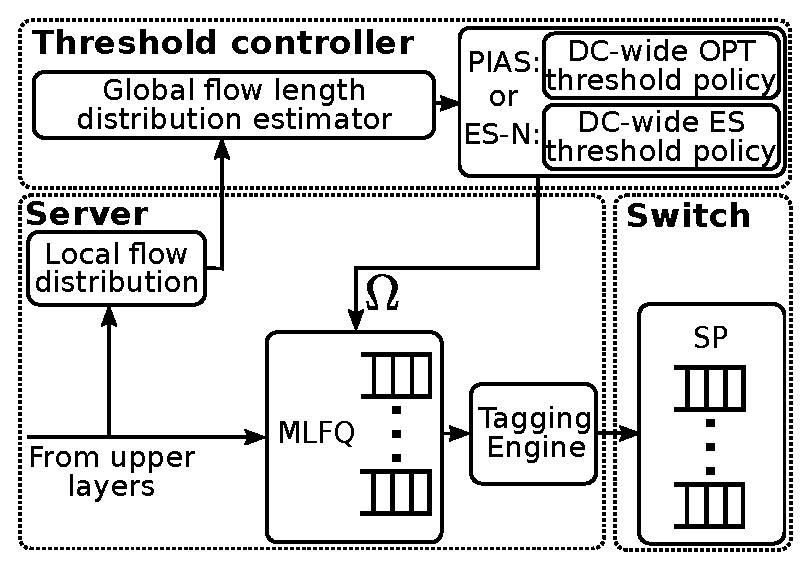
\includegraphics[width=0.6\linewidth]{Chapter4/Figures/pias-es_arch.eps}
%	\caption{High-level architecture of PIAS and of ES-$N$, with many PQs at the servers and at the switches.}
%	\label{fig:pias-es2}
%\end{figure}
\subsection{Host configuration}
\subsubsection{TCP}
% FIFO queues for UDP
% applications single socket for TCP
% no RTO change
% change in numbner of simultaneous configurations
% AW change instead of rate limiting because how is implemented omnet ...
\subsubsection{UDP}
% TCP & UDP, applications ot generate traffic, buffer sizing, window tcp, where to modify 
\subsection{DCTCP}
% general description of DCTCP, ECN confg, implementation details (?), RFC modification, testing

\section{Result analysis}
